\documentclass[12pt]{article}
\usepackage{fullpage}
\usepackage{setspace}
\usepackage{graphicx}
\usepackage{url}

\doublespacing

\title{Backbone-Store: An API for Automating Local Caching of Web Application
Data}
\author{Michael Stunes, Wolfe Styke, Fan (Frances) Zhang}

\begin{document}
\maketitle

\begin{abstract}
Efficiently storing web application data in the client's browser was a
challenging task until the recent HTML5 specification. With this new local storage spec, Web applications that require re-fetching the same data from a server
can see an improved load time by storing old data in the client's browser,
requiring only the new data to be retrieved from the server. In this paper, we present Backbone-Store: a local caching API that extends Backbone.js to help web developers easily store and reload a web application's data using the HTML5 localStorage API, and two different persistence strategies. To evaluate the API,  we analyze three simple applications to measure the performance characteristics of loading large
documents, medium-sized emails, and small notes from both the local storage on
the client's browser and from the server. As expected, we find that local storage performs
faster than loading the same data from the server. This time difference
increases for larger quantities of the same type of item, suggesting that local storage becomes more advantageous as the amount of data loaded by an application increases. %Furthermore, given that the threshold
%for users perceiving lag is about 100 milliseconds, we show that there are
%real-world use cases where loading data from a server would cause users to
%perceive lag, while loading the same data from localStorage would be perceived
%as instantaneous.
Futhermore, we examined the time required for an application to save data to the local storage, comparing the relative save-time performance of our two persistence strategies, and finding one to be more suitable for small updates to the application's data, and the other to be more suitable for larger updates.
\end{abstract}

\section{Introduction}

HTML5 presents new options for storing a web application's data in the client's
browser. The capacity for a web application to efficiently store information
that can be used the next time a user views the website presents two major
benefits. The first benefit is that the web application can store information
that it can use to help speed up the time it takes to present the user
interface for the web application. Users are sensitive to the time it takes a
web application to load, with slower applications causing users to navigate
away or think less of the site. The second benefit is that the web applications
can request less data from a server if it can store information that it
previously would have needed to fetch from the server. This allows a server to
fulfill more requests and thus reduces costs to maintain servers to meet a web
application's requests.

\section{Related Work}

There are several new client-side data storage options for web applications
using HTML5. Web SQL provides a database interface similar to SQLite and supports
transactions. However, Web SQL is not supported by all of the major browsers,
with Firefox in particular refusing to ever support Web SQL. HTML5 also offers two key-value storage options called sessionStorage and localStorage, that have a simple API (\verb=saveItem(key, value)=, \verb=getItem(key)=,
\verb=removeItem(key)=, and \verb=clear()=) for storing key-value pairs. 
Session storage stores data only while a user is viewing a website, and
automatically clears the data when a user navigates away from the site. Local
storage persists data until it is deleted by the application or by the user
clearing all of the website's information from the browser. In this paper, we use localStorage to implement our local caching strategies because it provides persistent storage (unlike sessionStorage) and is supported by all the major web browsers (unlike Web SQL). 

Backbone-store, the project described in this paper, presents a new way for web
application programmers to easily save their web application's data on the
client side to take advantage of the benefits of local storage (as described in the Introduction). This project is an extension of the pure-Javascript Backbone.js \cite{backbone} library, which is used by many companies (e.g., Four Square, Walmart Mobile, Pandora, Trello, etc.) to create web applications for browsers and mobile devices. Data
stored in Backbone.js applications are generally placed in either a Model
object or a Collection object, which is an ordered list of objects of one type
of Model. Backbone.js also provides View objects for managing the UI based on
the state of the Model or Collection objects.

Currently, web programmers wishing to employ local caching using Backbone.js would need to write a custom storage solution (including custom libraries and scripts tailored to the particular application) to save the data from each of their models and/or collections to HTML5's localStorage or another local storage option. Backbone-store simplifies this process by providing an API that automates the local caching process such that information from a saved model or collection can be reloaded into the
models and collections the next time the web application starts. With a few new
methods added to the Model and Collection objects, a web developer can choose
when a copy of a model's or collection's data should be stored, and when to
load saved data back into the application's models or collections. There is
also a choice of how the data is stored for collections of models. All models
can be stored as a bundle under one key in the localStorage (Strategy 1), or they can be
stored individually, with each model under its own key in the localStorage (Strategy 2).
These two local storage options provide flexibility for different use cases where one choice may be
significantly better than the other, depending on the number of items and
the amount of data being stored. We evaluate optimal conditions for each strategy in the Results section.

\section{The Problem Space}

We hypothesize that the browser's HTML5 localStorage persistent data storage
can be used by web applications to increase the speed required to load a web
application's user interface by providing faster access to different types of
items of required information.

Web applications vary in the amount and type of data they must request from a
server before presenting a user interface to a user. Two primary metrics
closely related to our project are the number of individual items requested,
and the size of each of these items. Some applications might require only a few
large items, such as showing a user a menu of large documents they can edit. On
the opposite end of both spectra, a note-taking application might request many
relatively small notes.

HTML5's localStorage presents a key-value storage API for storing a web
application's persistent information, using string keys and string or integer
values. However, Backbone.js collections and models store their data in
Javascript objects. Using the native JSON parse and stringify methods that
convert objects to strings and back again, the library we extend can easily
store the data from the models and collections as strings in localStorage, and
convert the stored strings back to their original object representations.

\section{Solution: Extending Backbone.js}

There are two primary ways to save Backbone.js collections consisting of many
models. One option is to turn the list of models into a JSON string and store
this information under a single key in localStorage. The other option is to
store each model in the collection under its own key. The main tradeoff in
these options is the time it takes to retrieve a single key from localStorage,
and the time it takes to parse a JSON string.

Our library extends Backbone.js by providing these two new persistence storage
options. For a web developer to use these options, the developer chooses a
default persistence strategy for all of their collections of models.
Additionally, the developer can choose a persistence strategy for each
individual collection. This allows the developer to easily specify a single
persistence strategy that will cover the majority of their needs, and only
change the strategy for the minority of collections that will use the
non-default option.

To store a model or a collection's models, a new instance method has been added
to the Backbone.Model and Backbone.Collection options called
``\verb=saveToStore=''. For models, this method simply saves the model's
attributes to the localStorage. For collections, this method uses the
persistence strategy identified by the collection to save the sorted list of
models into the localStorage. To load the data for a model or collection from
localStorage, a new method called ``\verb=loadFromStore='' has been added to
Backbone.Model and Backbone.Collection. For models, this simply loads the data
from localStorage into the model; for collections; this method identifies the
persistence strategy used by the collection and uses the correct retrieval
method to fetch the data from localStorage, parse it back into an array of
models, and add them to the collection.

\section{Contribution}

Our project makes two main contributions. First, we present an API that
automates local caching for web applications. This API will allow developers to
choose from two storage strategies for locally cached data:

\begin{enumerate}
\item Associate one key per collection
\item Associate one key per model in a collection
\end{enumerate}

Second, we conduct a performance evaluation of load times for data
stored locally (using the aforementioned two strategies) compared to data
stored remotely for three types of web applications that differ in data size
per item (70 bytes, 900 bytes, 3200 bytes) and data quantity (10, 50, 100, 200,
300 items per collection) and highlight conditions where local storage is most
advantageous.

We find that our API provides superior load performance for data
stored locally vs.\ remotely under all data sizse and quantity conditions except
for the case of loading many small items. Furthermore, we find that our
implementation of local caching exhibits the greatest speedup when data is
stored using the first strategy, with one key-value pair per collection. This
suggests that local caching is most advantageous for applications that load
data of larger size, and moderate to large quantity.

\section{Evaluation}

To evaluate the benefits of Backbone-store, we built three test applications to
understand how our solution handled three different sizes of items requiring
storage. To test large items that might represent a document, we used five
paragraphs of Lorem ipsum, totaling 3265 characters per item (~3200 bytes). To examine
medium size items such as emails, we used one paragraph of Lorem ipsum,
totaling 905 characters per item (~900 bytes) . To examine smaller items such as personal
notes, we used a short string of 70 characters (~70 bytes). These character lengths are the
length of the JSON string that represents each item. The three applications
performed the same task: 
\begin{enumerate}
\item load some number of a particular type of item (e.g., doc, email, note) from
local storage
\item load some number of a particular type of item (e.g., doc, email, note) from the server
\item record the load time.
\end{enumerate}

Note that Step 1 and 2 are separated by a delay so as not to overlap in
execution and skew the load time.

Each of the three web applications records how long it takes the application to
load the data for each of the three test applications. For the time it takes to
load data from the server, the timer is started just before an Ajax request
asks the server for the data. When the data returns from the server, it is
loaded into a Backbone.Collection object, and the timer is stopped after this
is complete. To record the time to load the same data from local storage, the
timer is started when just before the \verb=loadFromStore= method is called by
a collection. The data is then fetched from local storage and parsed from a JSON
string into an array of objects, which is then added to the collection before
finally stopping the timer.

We created a simple server using Node.js \cite{node} for our test applications. Our timing
application presented a blank page which loaded a particular number of items
for each of the three types of models into collections from both localStorage
and from server requests. Three request URLs allowed the web application to use
Ajax to query the server for the data needed for each type of model. To easily
collect a large enough sample size of timing data, we had the server record
responses from the web application and print out batches of times for 15
requests to a CSV file. This allowed us to rapidly collect timing data for each
scenario.

Finally, we also tested update times for our two local storage strategies, by
creating collections with different numbers of items and measuring the time to
save each collection to local storage. Also, we believe that our two strategies
will behave differently in different situations (i.e., saving an entire
collection for the first time, and saving a collection again after having
changed or added only a few models); we test this by measuring the time to
resave the collection after adding one new model. We predict that the
one-key-per-model local storage strategy will allow faster updates, by making
it possible to save only those models that were changed or added since the last
save.

\section{Results}

Below we present results that measure the load times of data from both local
storage and the server for three types of applications, listed here, in
decreasing order of data size:

\begin{enumerate}
\item Documents
\item Email
\item Notes
\end{enumerate}

We load the data from each application in varying quantities (10, 50, 100, 200,
300 items per collection) and show that local caching performs faster than data
loaded from the server (except for collections of small items, where the gain
becomes negligible, most likely because of the overhead involved in retrieving
items from the local store).

\begin{figure}[th]
  \centering
  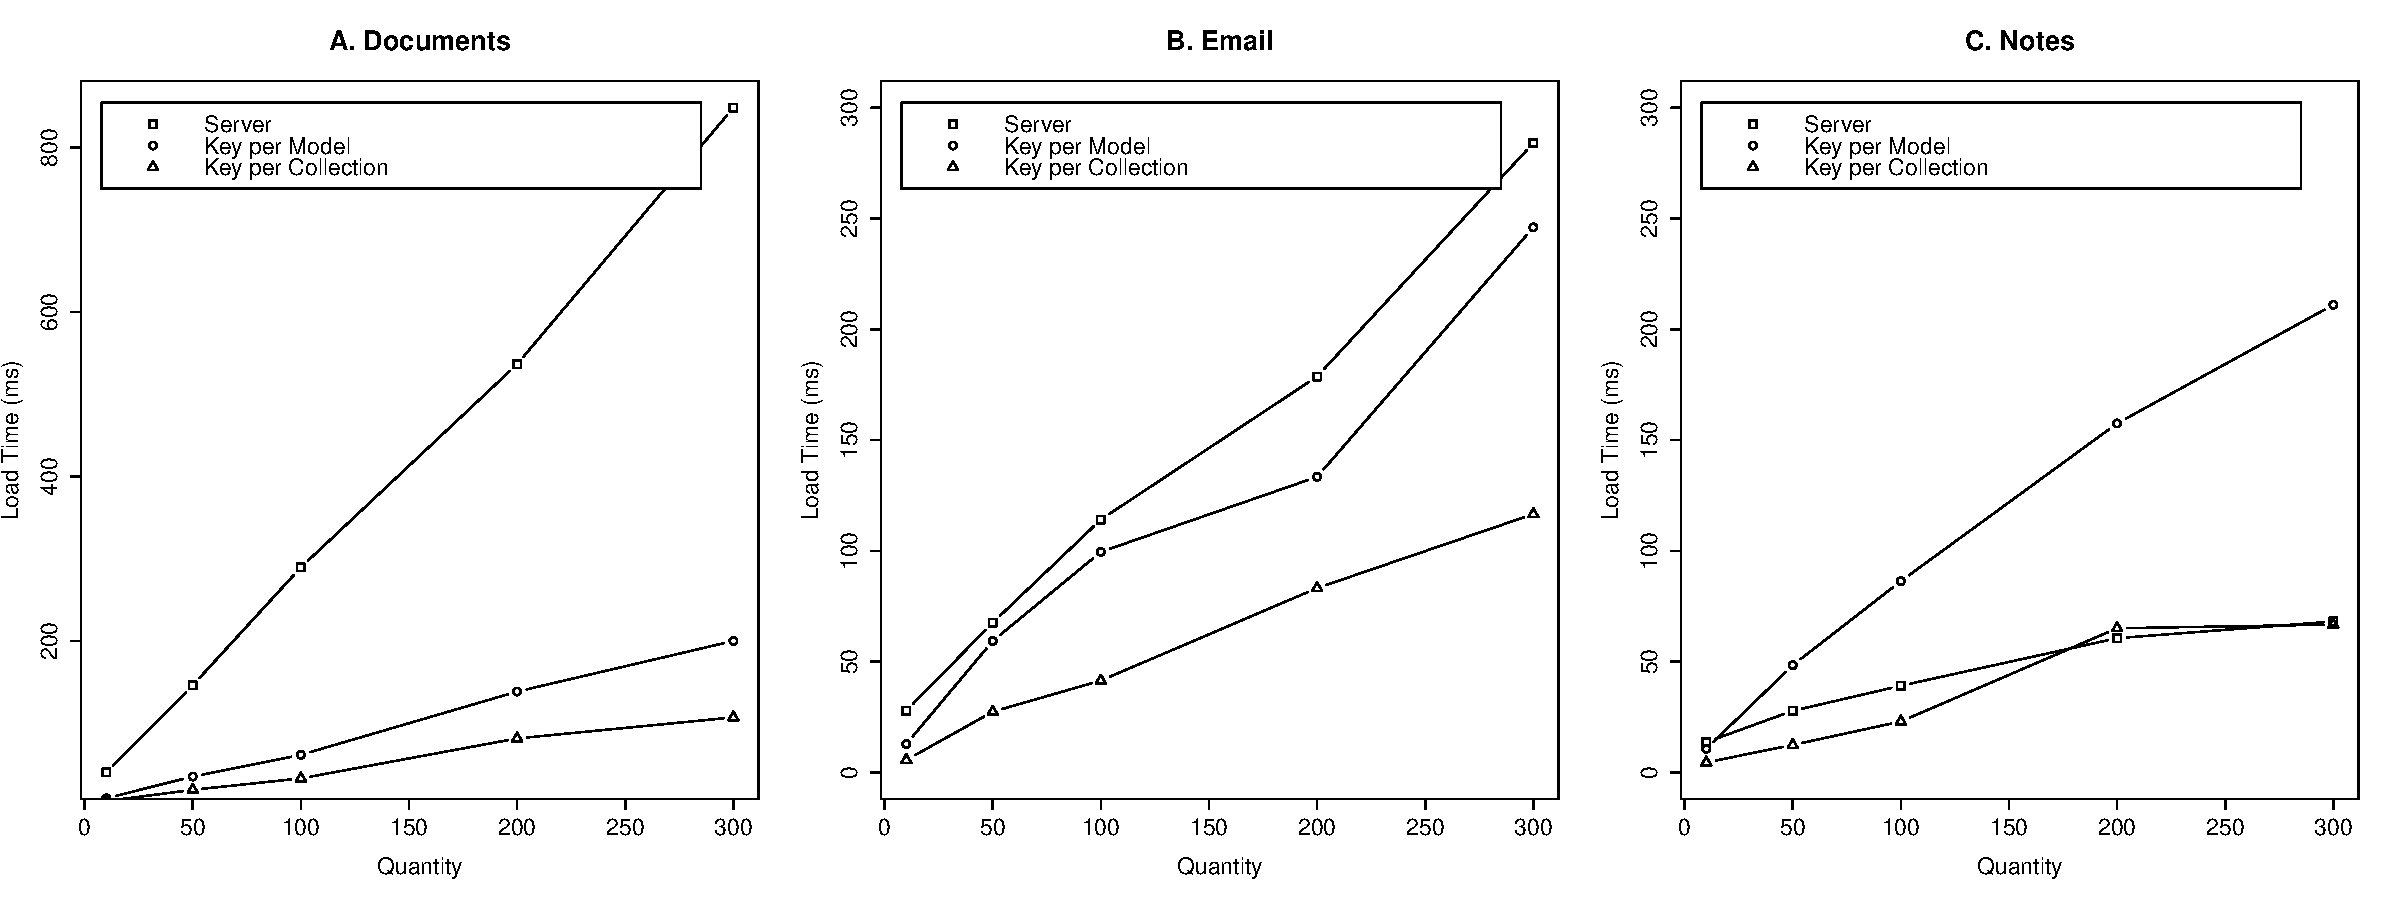
\includegraphics[width=\textwidth]{lines.pdf}
  \caption{Load time as a function of collection size, for each persistence
  method and item size.}
  \label{fig:line}
\end{figure}

Loading large items, such as documents, from the local storage (shown in Figure
\ref{fig:line}A) gives the results that we expect. Load times for both
local storage strategies, and from the server, grow linearly with the number of
items in the collection, and thus with the amount of data retrieved. Both local
persistence methods are faster than retrieving items from the local storage;
the one-key-per-model method is slightly slower than the one-key-per-collection
method due to the additional overhead of retrieving each model from the local
storage separately.

Repeating the same tests with medium-sized items, such as emails (shown in
Figure \ref{fig:line}B), shows similar results; however, the difference in
speed here is less pronounced. This is due to the constant overhead imposed by
accessing the local storage; in the documents example, this overhead is masked
by the linear overhead of retrieving large amounts of data from storage. As in
the previous example, the one-key-per-model method is still slightly slower,
due to additional overhead from retrieving each model from the storage
separately.

Finally, repeating these tests with very small items, such as notes (shown in
Figure \ref{fig:line}C), shows different results: in this case, loading from
local storage is negligibly faster, with the difference becoming smaller for
larger collections. With very small items in the collection, the additional
overhead of the one-key-per-model method becomes large enough to outweigh the
load-time benefits of local storage.

It is of note that users typically perceive lag in an interface when an
operation takes more than 100 milliseconds to complete. In all of our tests,
the key-per-model persistence strategy was able to keep the load time for the
collection below or very near 100 ms, meaning that users would perceive the
load time as nearly instantaneous. The load time from the server is much
higher, so users will perceive noticeable lag while waiting for the application
to load. This demonstrates that our extension provides application users with
an improved user experience, due to faster application load times.

\begin{figure}[th]
  \centering
  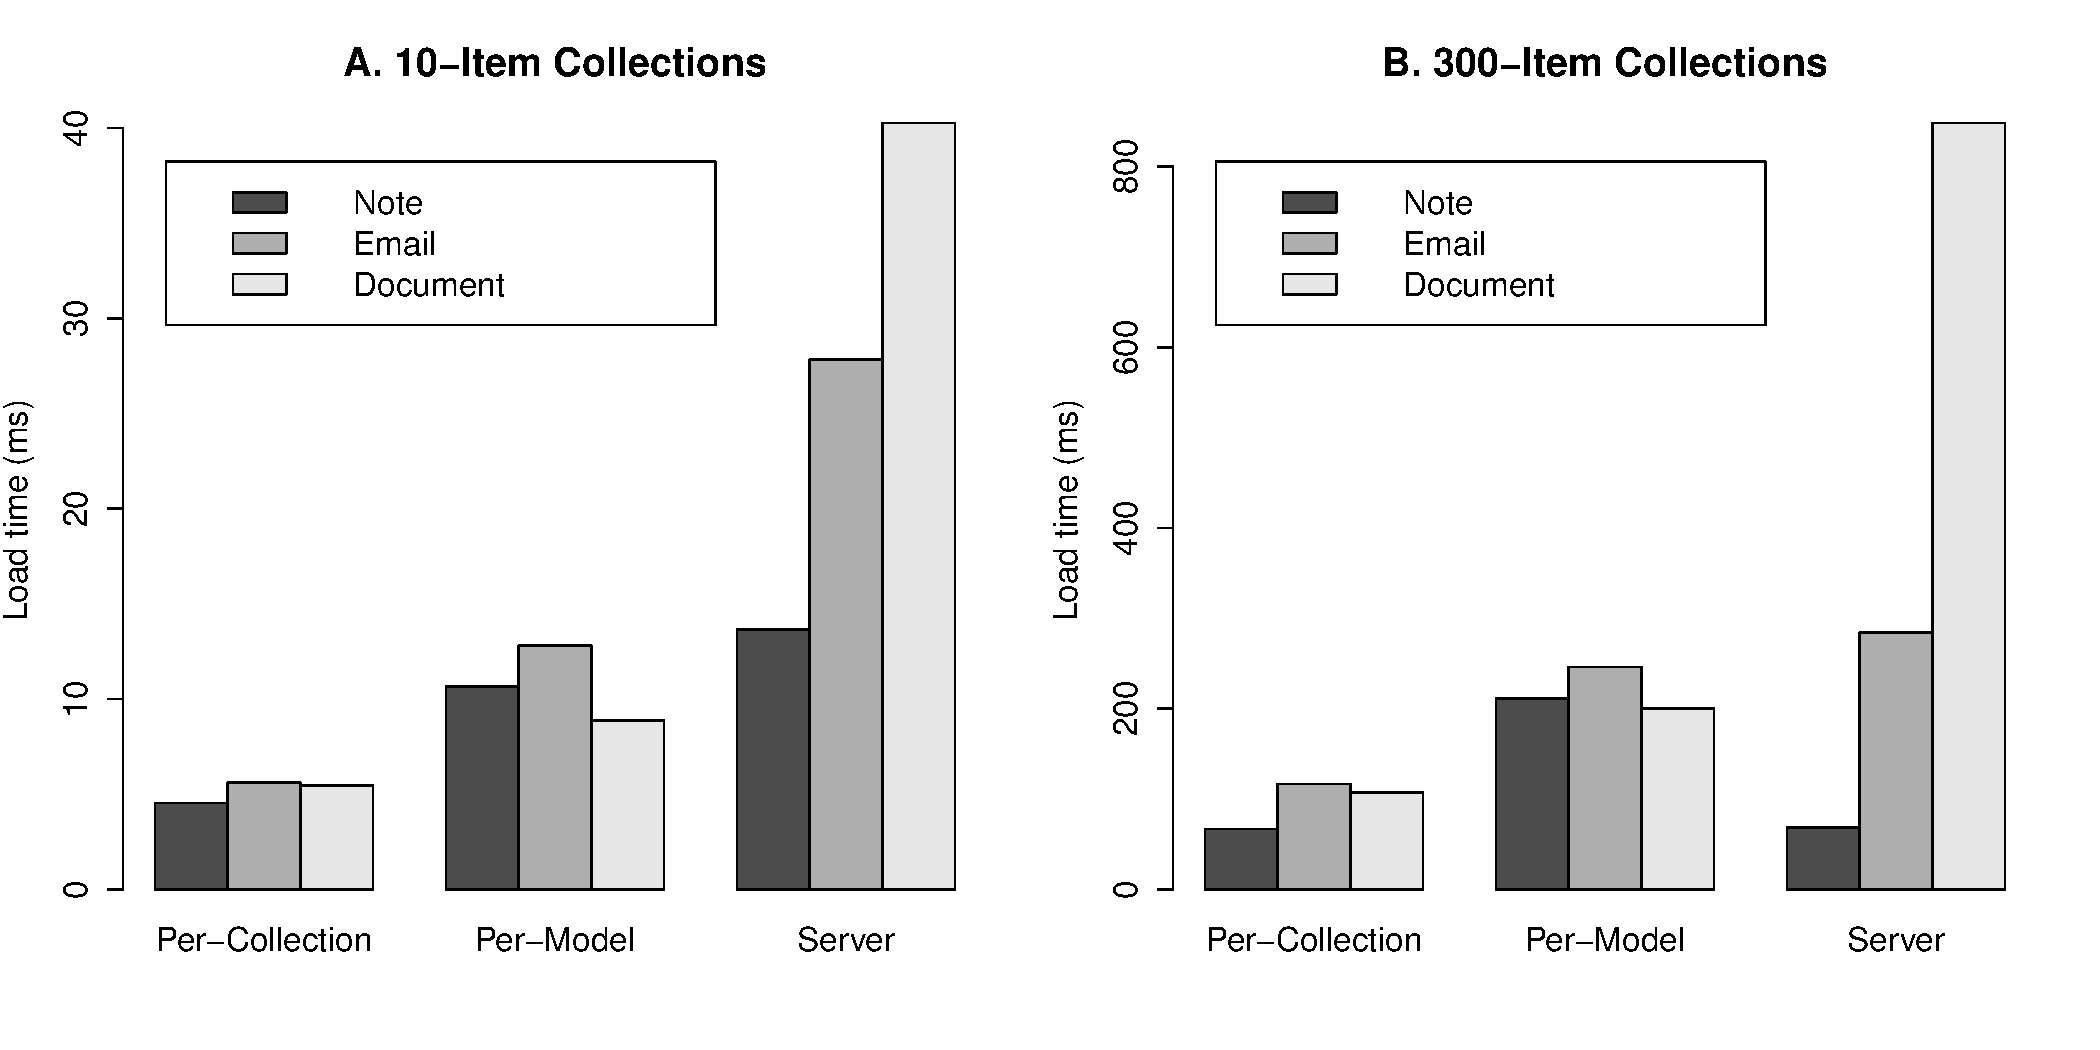
\includegraphics[width=\textwidth]{bars.pdf}
  \caption{Load time as a function of item size, for each persistence method
  and two different collection sizes.}
  \label{fig:bar}
\end{figure}

Figure \ref{fig:bar} shows the effect of the size of individual items on the
time to load collections both from storage and from the server. As expected,
load times from the server are generally higher; also, the difference in load
time due to the size of the individual items is much more pronounced when
loading from the server. Differences in load times due to item size for
retrieving collections are much less pronounced when loading from local
storage; again, much of the overhead in loading locally is fixed, and caused
simply by accessing the local store.

\begin{figure}[th]
    \centering
    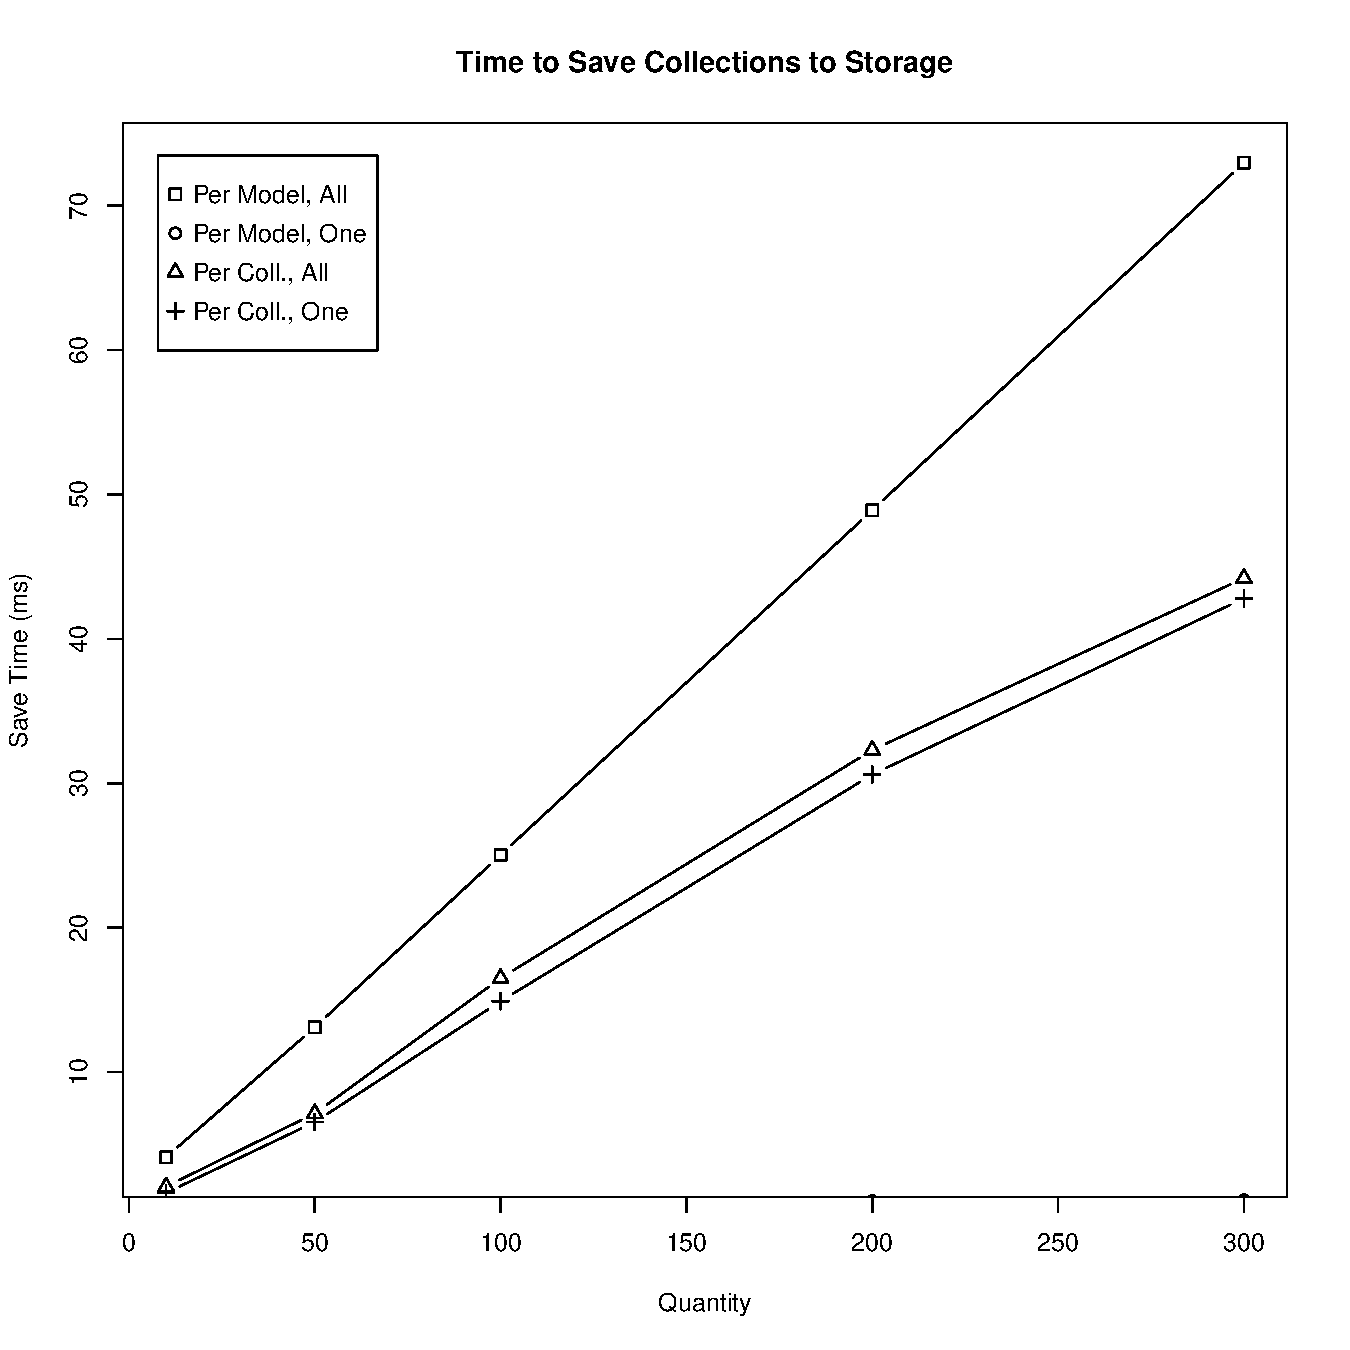
\includegraphics[width=0.7\textwidth]{save.pdf}
    \caption{Save time as a function of collection size, for each persistence
    method.}
    \label{fig:save}
\end{figure}

Figure \ref{fig:save} shows the elapsed time for saving a collection of
document-size items into localStorage, while varying the number of items in the
collection. For both persistence strategies, the time to save the entire
collection grows linearly with the size of the collection as expected;
furthermore, the one-key-per-model strategy takes longer to save an entire
collection, because of the overhead involved in writing many keys to the
localStorage.

Also, as expected, the time to resave the collection after adding one model is
much lower (approx. 1 ms in every case) for the one-key-per-model strategy, as
we are able to save only that model to the localStorage. For the
one-key-per-collection strategy, the time to save one more model is
approximately the same as the time to save all of the models, because this
strategy must write the entire collection to localStorage in either case.

\section{Conclusion}

This report described our extension for the Backbone.js library, which
simplifies the task of persisting a collection of data models to a web
browser's local storage, in order to facilitate faster load times and reduced
server load. This extension provides an API to facilitate saving and loading
collections on demand, using one of two different persistence strategies. We
tested our extension using three different demo applications, with different
characteristics for the data that is being used by the application. Our tests
varied both the number of data items in a single collection and the size of
each data itme, to simulate a number of different application scenarios. Our
tests showed that our extension is effective at reducing the load times in many
different scenarios, resulting in an improved experience for the application
user.

\bibliographystyle{plain}
\bibliography{paper}

\end{document}
